%
% subsystems.tex
%
% Copyright (C) 2021 by SpaceLab.
%
% GOLDS-UFSC Documentation
%
% This work is licensed under the Creative Commons Attribution-ShareAlike 4.0
% International License. To view a copy of this license,
% visit http://creativecommons.org/licenses/by-sa/4.0/.
%

%
% \brief Subsystems chapter.
%
% \author Gabriel Mariano Marcelino <gabriel.mm8@gmail.com>
%
% \institution Universidade Federal de Santa Catarina (UFSC)
%
% \version 0.1.0
%
% \date 2020/06/06
%

\chapter{Subsystems} \label{ch:subsystems}

\begin{figure}[!ht]
    \begin{center}
        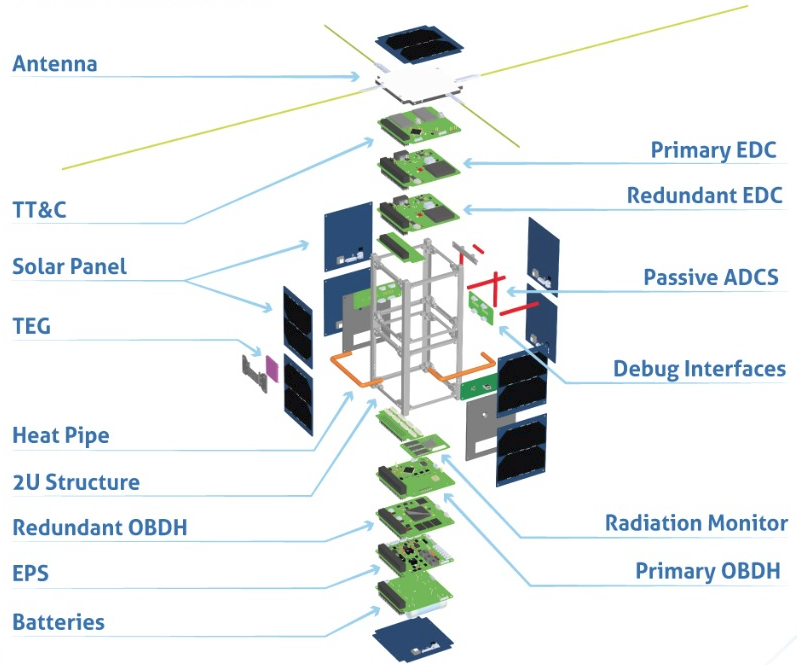
\includegraphics[width=\textwidth]{figures/exploded-view}
        \caption{Exploded view of the GOLDS-UFSC satellite.}
        \label{fig:exploded-view}
    \end{center}
\end{figure}

\section{On-Board Data Handling}

OBDH\nomenclature{\textbf{OBDH}}{\textit{On-Board Data Handling}.} \cite{obdh2}

\section{Telemetry, Tracking and Command Module}

TTC\nomenclature{\textbf{TTC}}{\textit{Telemetry, Tracking and Command Module}.} \cite{ttc}

\subsection{Antenna Module}

.

\section{Electrical Power System}

EPS\nomenclature{\textbf{EPS}}{\textit{Electrical Power System}.} \cite{eps2}

\subsection{Battery Module}

\cite{bat4c}

\section{Attitude Determination and Control System}

ADCS\nomenclature{\textbf{ADCS}}{\textit{Attitude Determination and Control System}.}

\section{Mechanical Structure}

.

\section{Interconnection Modules}

\subsection{PC-104 Interconnection Boards}

\cite{pc104-boards}

\subsection{External Connection Boards}

\cite{iip}

\section{Payloads}

\subsection{Environmental Data Collection}

EDC\nomenclature{\textbf{EDC}}{\textit{Environmental Data Collection}.} \cite{edc}
